\subsection{Background}
\begin{frame}[allowframebreaks]{Why collaborative learning is important?}

    \begin{figure}[tb]
        \begin{center}
            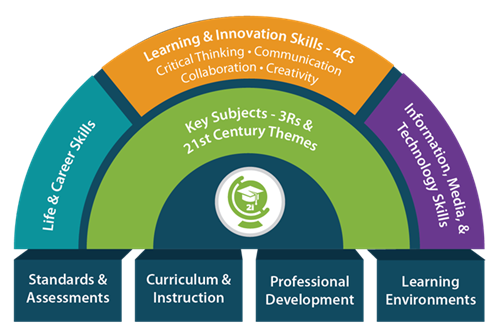
\includegraphics[width=70mm]{images/p21centuryskills.png}
        \end{center}
        \caption{Partnership for 21st century learning. Source: https://www.battelleforkids.org/networks/p21}
        \label{intro::p21}
    \end{figure}

    \begin{itemize}
        \item Collaboration is one of the four-essential skills in 21st century skills
        \item The advancement of technology and rapidly changing environment require 
        collaborative works of multidisciplinary experts to solve complex problems effectively
        \item Collaboration does not merely happen just because individuals are co-present
        \item It is indeed necessary to practice collaboration in the classroom
    \end{itemize}
\end{frame}

\begin{frame}[allowframebreaks]{Designing learning activities to encourage collaboration}
    \begin{itemize}
        \item Students' interactions play a fundamental role in collaborative learning 
        \cite{Baines2009ImprovingStudy,Webb2009TheClassroom}
        \item Various instructional strategies are employed to encourage learners to collaborate 
        (i.e. scripts, scenarios, representational tools).
        \item During collaboration individual learners need to make a continuous effort 
        to construct and maintain group-shared knowledge \cite{Roschelle1995TheSolving}. 
        \item They may have forgotten prior discussion or feeling difficult to remember 
        what they have discussed or co-constructed \cite{Jeong2016SevenHelp}.
    \end{itemize}
\end{frame}

\begin{frame}[allowframebreaks]{Collaborative concept mapping}

    % add concept map figures
    \begin{figure}[tb]
        \begin{center}
            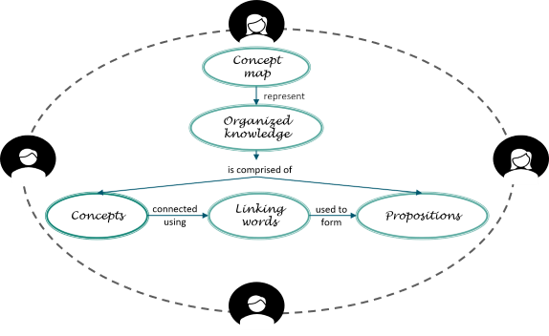
\includegraphics[width=70mm]{images/ccm.png}
        \end{center}
        \caption{Collaborative concept map}
        \label{intro::ccm}
    \end{figure}
    
    \begin{itemize}
        \item An external representation tool assist the learner in articulating 
        and maintaining shared focus during discourse \cite{Fischer2002FosteringTools,Suthers2006TechnologyCSCL,vanBoxtel2002CollaborativeDiscourse}
        \item A concept map is a graphical tool for organizing and representing knowledge which consists of concepts and relationships among these concepts to facilitate meaningful learning \cite{novak1984learning}.
        \item A concept map has been widely used as a representational tool to facilitate group
        discussion, as well as to communicate complex ideas 
        \cite{Fischer2002FosteringTools,Gracia-Moreno2017CollaborativeWorkspaces,Suthers2006TechnologyCSCL,vanBoxtel2000CollaborativeKnowledge}

        \item Previous studies posited that concept mapping has a positive effect on both students’ attitudes and learning achievements \cite{Basque2006CollaborativeTrends,Czerniak1998TheScience}.
    \end{itemize}
\end{frame}

\begin{frame}[allowframebreaks]{Collaborative concept mapping with KB approach}

    % add concept map figures
    \begin{figure}[tb]
        \begin{center}
            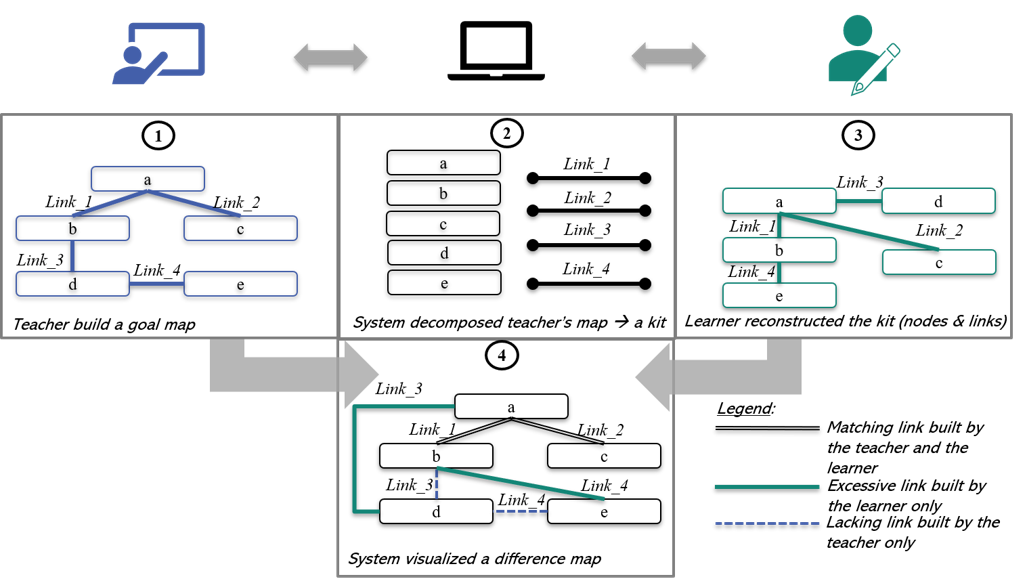
\includegraphics[width=90mm]{images/kb_flow.png}
        \end{center}
        \caption{Learning activity with KB concept map}
        \label{intro::kbmap}
    \end{figure}
    
    \begin{itemize}
        \item The KB is a re-constructional closed-ended approach to concept mapping
        activity in which students construct a map based on predefined nodes and
        links extracted from an expert's map \cite{Hirashima2015,Hirashima2019ReconstructionalReconstruction}. 
        \item The KB approach enables teacher to confirm students' understanding
        of the information delivered by him/her. 
        \item Concept mapping activity with KB approach allow ones to externalize 
        their understanding on the perspective of other.

    \end{itemize}
\end{frame}

\begin{frame}[allowframebreaks]{Empathetic collaboration with KB approach}
    \begin{itemize}
        \item Effective collaboration is fueled by empathy - \emph{an awareness of
        others and an ability to detect their emotions and 
        understand their perspective.} 
        \item To come up with truly  innovative solutions requires new ideas. 
        \item To bring new ideas 
        to light requires seeking a diversity of perspectives 
        and creating a welcoming space for people to share 
        their ideas without fear of judgment.
        % \item Intellectual empathy: recognizing the need to imaginatively
        % put oneself in the place of others to genuinely 
        % understand them
        \item Therefore, we implemented the KB approach during 
        collaborative concept mapping to support empathetic communication and 
        build a shared knowledge.
    \end{itemize}

\end{frame}

\begin{frame}[allowframebreaks]{Reciprocal Kit Build (RKB)}

    \begin{figure}[tb]
        \begin{center}
            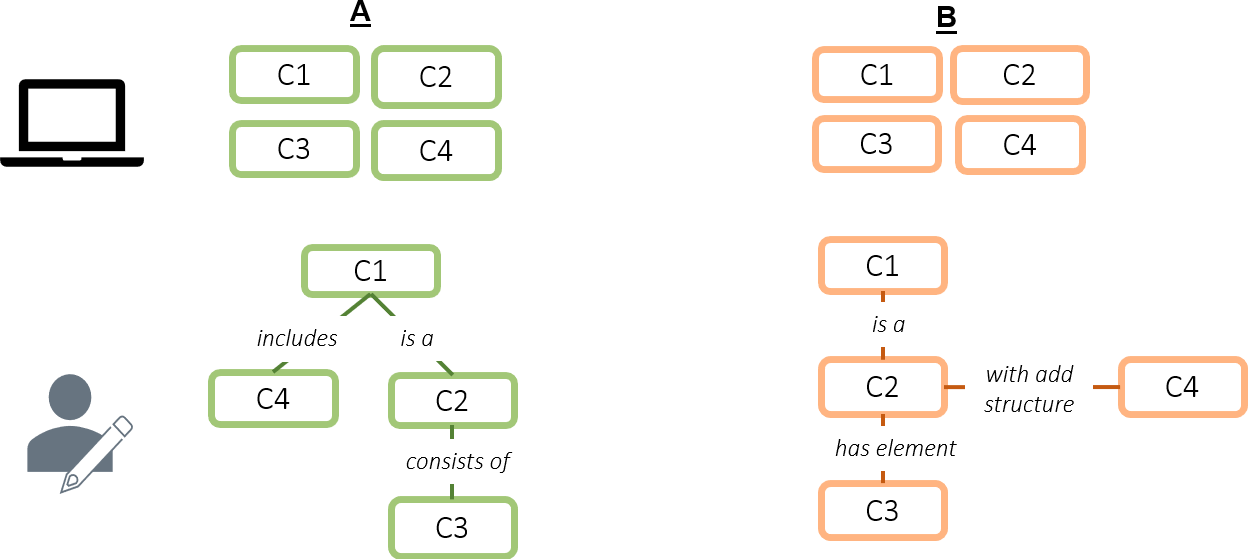
\includegraphics[width=100mm]{images/RKB_p1.pdf}
        \end{center}
        \caption{\emph{Individual phase} -- Initial map construction}
        \label{intro::rkb_p1}
    \end{figure}
    
    \begin{figure}[tb]
        \begin{center}
            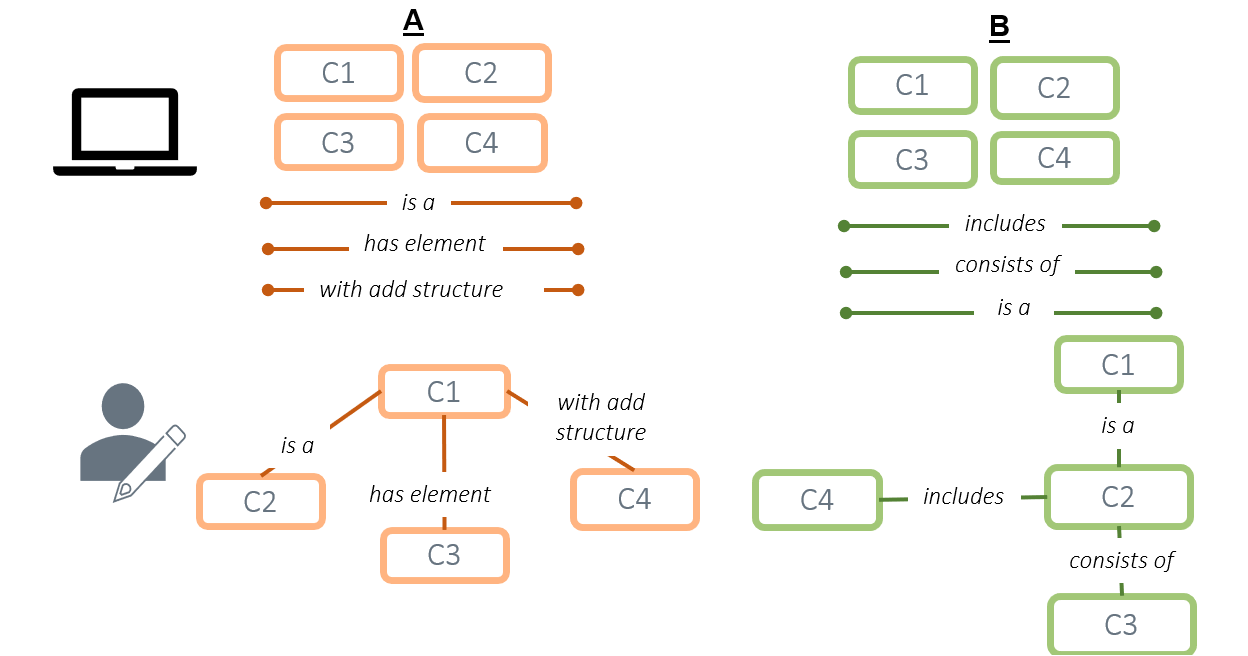
\includegraphics[width=100mm]{images/RKB_p2.pdf}
        \end{center}
        \caption{\emph{Individual phase} -- Re-constructional map building}
        \label{intro::rkb_p2}
    \end{figure}
    
    \begin{figure}[tb]
        \begin{center}
            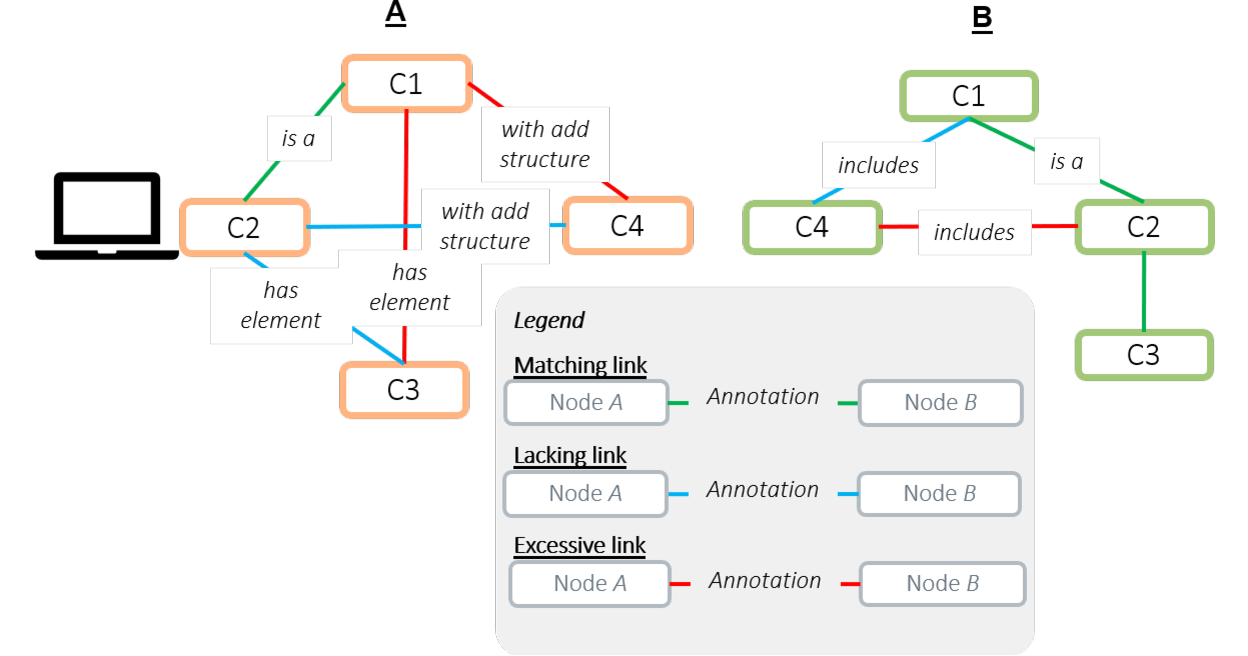
\includegraphics[width=100mm]{images/RKB_p3.pdf}
        \end{center}
        \caption{\emph{Collaborative phase} -- Visualization of map similarities and differences \& group discussion}
        \label{intro::rkb_p3}
    \end{figure}
    
    \begin{figure}[tb]
        \begin{center}
            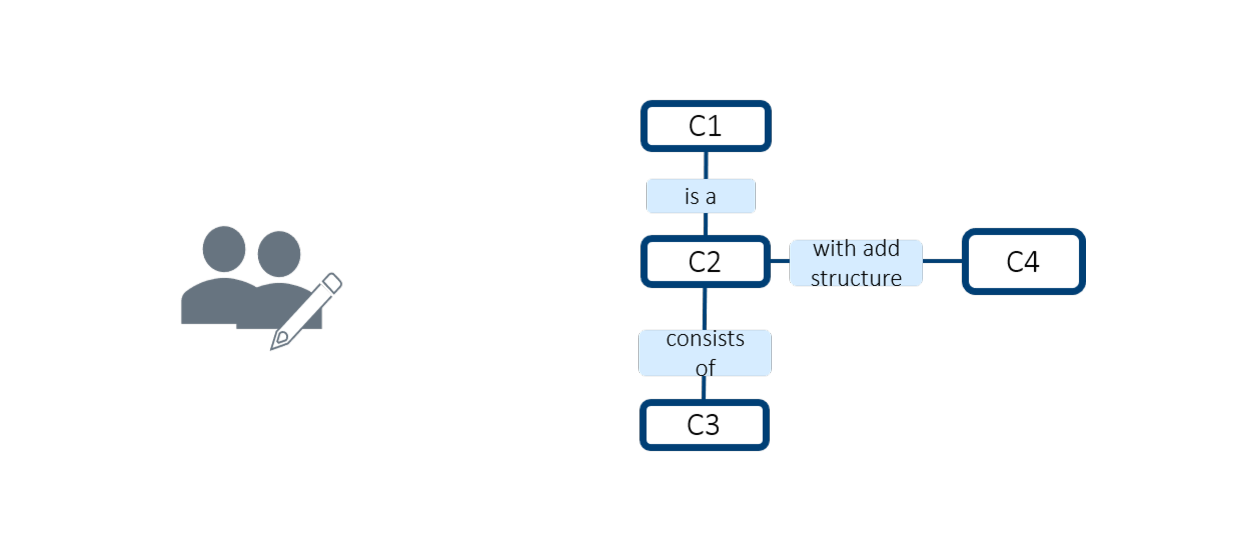
\includegraphics[width=100mm]{images/RKB_p4.pdf}
        \end{center}
        \caption{\emph{Collaborative phase} -- Group map construction}
        \label{intro::rkb_p4}
    \end{figure}
    
 
\end{frame}


\subsection{Challenges}

\begin{frame}{Findings of the previous studies}
    \begin{itemize}
        \item Initial studies showed that the RKB approach promoted productive
        discussion between partners compared to the group without reconstruction
        and difference map-supported discussion
        \cite{Wunnasri2018ReciprocalUnderstanding}. 
        \item The RKB map also encouraged the pair of partners to understand each other based on the similarity
        score of the individual's map after discussion
        \cite{Wunnasri2018ReciprocalCollaboration}. 
        \item Their findings demonstrated that the RKB can be used to share understanding as preparation for
        collaboration. 
        \item However, they have not evaluated the effect of applying
        this approach to collaborative knowledge building, so far. 
        
    \end{itemize}
\end{frame}

\begin{frame}[allowframebreaks]{Remaining problems}
    \begin{enumerate}
        \item \textcolor<1>{blue}{Collaborative product evaluation.} 
        After following RKB activities, 
        whether or not high-quality group products could be achieved is still 
        a remaining question.  
        \item \textcolor<1>{blue}{Students' perspective toward the activities.} 
        Applying new learning activity 
        in a practical classroom as a part of real teaching activity need to 
        consider the perspective of students. An evaluation regarding 
        students acceptance of this activity is as important as the learning product itself. 
        \item \textcolor<1>{blue}{Group formation effect on collaboration.}
        Researches suggest that 
        when forming a group, we need to consider several factors, e.g. similarity 
        of individual knowledge.
        To what extent, this factor would influence collaboration need to be investigated.  By doing so, we could determine appropriate group settings. 
        \item \textcolor<1>{blue}{Finding factor to consider for designing support function for collaboration.}
        During RKB session, the learners build an individual map 
        two times. Which part of KB is a stronger predictor to estimate group 
        product? Whether similarity of individual knowledge or comprehension
        on partner's comprehension is a strong predictor to
        estimate the final group product? 
    \end{enumerate}
\end{frame}

\subsection{Research objectives}
\begin{frame}[allowframebreaks]{Research objectives}
    This study aims to identify the effect of the RKB approach
    for collaborative learning
    The purposes of this study are as follow:
    \begin{itemize}
        \item to identify the effect of the RKB approach on collaborative 
              concept mapping in a practical classroom.
        \item to investigate how individual differences in prior knowledge 
              may influence collaborative-learning effectiveness 
              (e.g. transfer of knowledge, lost knowledge, group product) 
              and the students' feelings about the learning process itself. 
        \item to investigate how individual prior knowledge convergence and comprehension 
            levels through reconstruction may potentially predict the final 
            collaborative product. 
    \end{itemize} 
\end{frame}